\documentclass{article}

\usepackage{graphicx}
\usepackage{tikz}
\usepackage{tikzsymbols}
\usetikzlibrary{calc,patterns,shapes.geometric}
\pagestyle{empty}
\usepackage[margin=0pt]{geometry}
\geometry{papersize={14in,12in}}

\def\centerarc[#1](#2)(#3:#4:#5){\draw[#1] ($(#2)+({#5*cos(#3)},{#5*sin(#3)})$) arc (#3:#4:#5);}

\begin{document}
	\begin{figure}
		\centering
		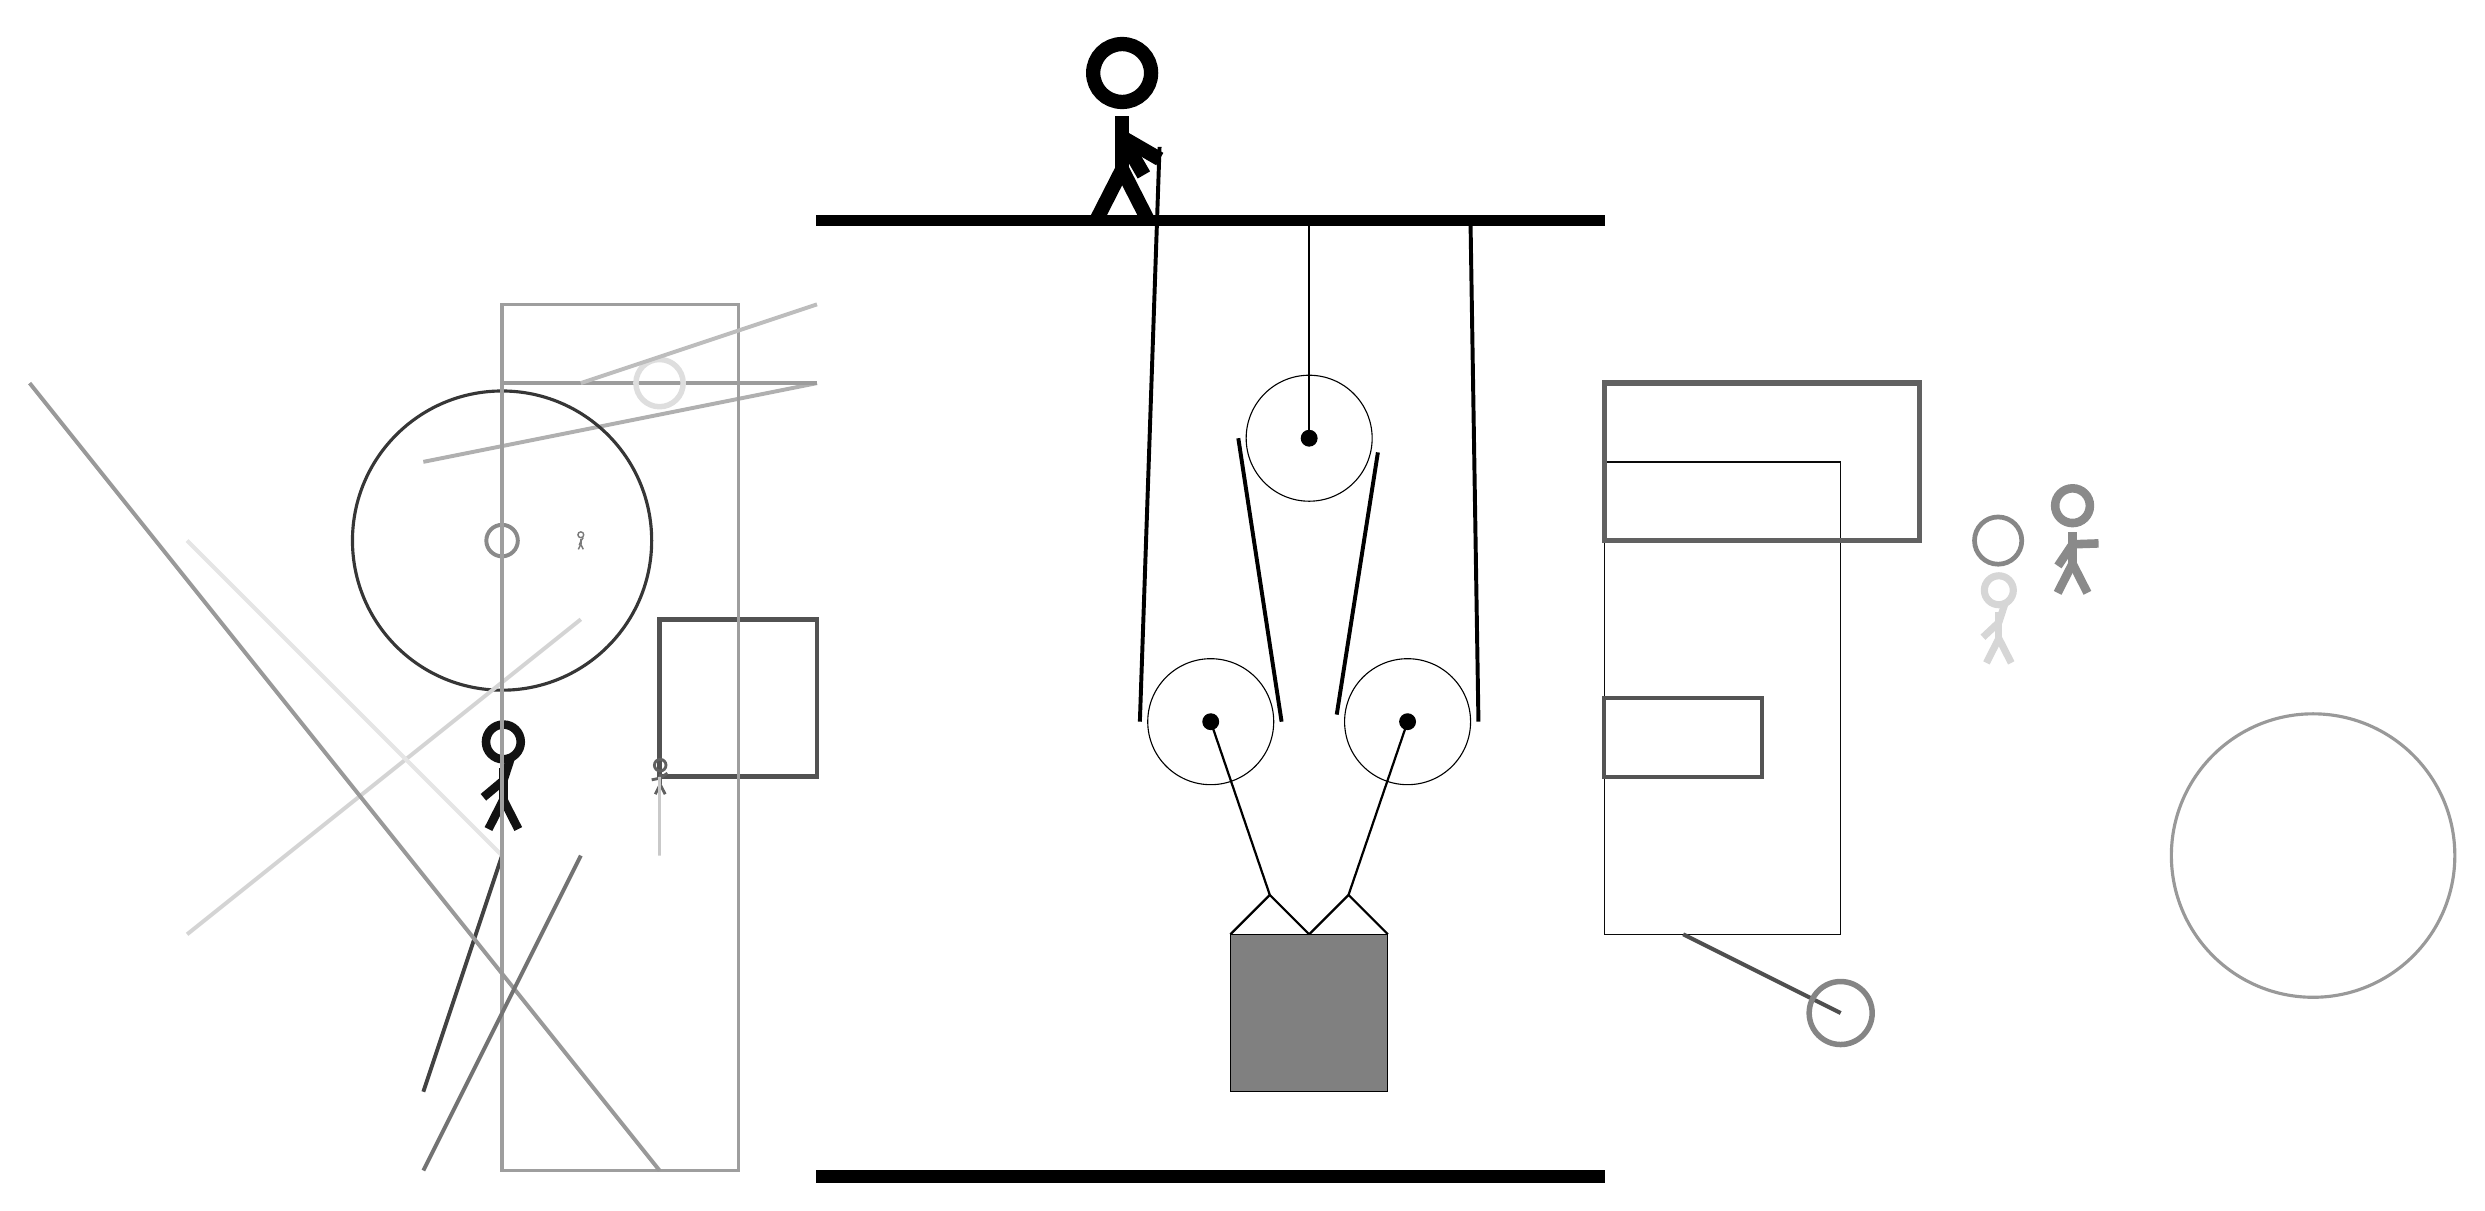
\begin{tikzpicture}
			%%%%% START %%%%%
			
			\draw[fill=black] (-4, 9) rectangle (6, 9.125);
			
			\draw [line width=0.6mm, color=black!47](11, 5) circle (0.3);
			
			\draw[line width=0.5mm, color=black!31](-9, 6) -- (-4, 7);
			\draw[line width=0.5mm, color=black!39](-4, 7) -- (-8, 7);
			\node[line width=0.2mm, color=black!93] at (-8, 2) {\Strichmaxerl[6][40][72]};
			
			\draw[line width=0.6mm, color=black!68] (-6, 4) rectangle (-4, 2);
			\node[line width=0.6mm, color=black!46] at (12, 5) {\Strichmaxerl[6][56][2]};
			\draw [line width=0.4mm, color=black!79](-8, 5) circle (1.9);
			
			\draw[line width=0.2mm, color=black!96] (6, 6) rectangle (9, 0);
			\draw[line width=0.5mm, color=black!69](7, 0) -- (9, -1);
			\draw [line width=0.5mm, color=black!46](-8, 5) circle (0.2);
			\draw [line width=0.4mm, color=black!40](15, 1) circle (1.8);
			\node[line width=0.5mm, color=black!16] at (11, 4) {\Strichmaxerl[5][43][72]};
			\draw[line width=0.5mm, color=black!17](-7, 4) -- (-12, 0);
			\draw [line width=0.7mm, color=black!13](-6, 7) circle (0.3);
			\draw[line width=0.5mm, color=black!74](-8, 1) -- (-9, -2);
			\draw[line width=0.5mm, color=black!10](-8, 1) -- (-12, 5);
			\draw[line width=0.4mm, color=black!38] (-5, 8) rectangle (-8, -3);
			
			\draw[line width=0.5mm, color=black!26](-7, 7) -- (-4, 8);
			\draw[line width=0.7mm, color=black!62] (6, 5) rectangle (10, 7);
			\draw[line width=0.5mm, color=black!40](-6, -3) -- (-14, 7);
			\node[line width=0.7mm, color=black!62] at (-6, 2) {\Strichmaxerl[2][12][34]};
			\node[line width=0.3mm, color=black!52] at (-7, 5) {\Strichmaxerl[1][68][57]};
			
			\draw[line width=0.4mm, color=black!21] (-6, 1) rectangle (-6, 2);
			\draw[line width=0.5mm, color=black!55](-9, -3) -- (-7, 1);
			\draw[line width=0.5mm, color=black!67] (6, 3) rectangle (8, 2);
			
			\draw [line width=0.7mm, color=black!48](9, -1) circle (0.4);
			
			\draw (1, 2.7) circle (0.8);
			\draw[fill=black] (1, 2.7) circle (0.1);
			
			\draw (2.25, 6.3) circle (0.8);
			\draw[fill=black] (2.25, 6.3) circle (0.1);
			\draw[thick] (2.25, 6.3) -- (2.25, 9);
			
			\draw (3.5, 2.7) circle (0.8);
			\draw[fill=black] (3.5, 2.7) circle (0.1);
			
			\draw[thick] (3.5, 2.7) -- (2.75, 0.5);
			\draw[thick] (1, 2.7) -- (1.75, 0.5);
			\draw[thick]  (1.25, 0) -- (1.75, 0.5) -- (2.25, 0);
			\draw[thick]  (2.25, 0) -- (2.75, 0.5) -- (3.25, 0);
			\draw[fill=black!50] (1.25, 0) rectangle (3.25, -2);
			
			\draw[line width=0.5mm] (0.35, 10) --  (0.1, 2.7);
			\centerarc[line width=0.5mm](1, 2.7)(180:360:0.9);
			\draw[line width=0.5mm] (1.9, 2.7) -- (1.35, 6.3);
			\centerarc[line width=0.5mm](2.25, 6.3)(-20:180:0.9);
			\draw[line width=0.5mm](3.123, 6.12) -- (2.6, 2.79);
			\centerarc[line width=0.5mm](3.5, 2.7)(160:360:0.9);
			\draw[line width=0.5mm](4.4, 2.7) -- (4.3, 9);
			
			\node at (-0.07, 10.2) {\Strichmaxerl[10][120][-30]};
			
			\draw[fill=black] (-4, -3) rectangle (6, -3.15);
			
			%%%%% END %%%%%
		\end{tikzpicture}
	\end{figure}	
\end{document}